%%%%%%%%%%%%%%%%%%%%%%%%%%%%%%%%%%%%%%%%%%%%%%%%%%%
%
%  New template code for TAMU Theses and Dissertations starting Fall 2016.
%
%  Author: Sean Zachary Roberson
%	 Version 3.16.09
%  Last updated 9/12/2016
%
%%%%%%%%%%%%%%%%%%%%%%%%%%%%%%%%%%%%%%%%%%%%%%%%%%%
%%%%%%%%%%%%%%%%%%%%%%%%%%%%%%%%%%%%%%%%%%%%%%%%%%%%%%%%%%%%%%%%%%%%%%
%%                           SECTION IV
%%%%%%%%%%%%%%%%%%%%%%%%%%%%%%%%%%%%%%%%%%%%%%%%%%%%%%%%%%%%%%%%%%%%%



\chapter{DYNAMICS EXAMPLES \label{sect:dyn}}

Reactor dynamics is the study of the time-dependent behavior of reactors as an entire system. This study includes the physical nature of neutrons and their feedback with power generation.  This feedback includes coupling with other physical properties such as temperature, fluids, material dynamics, etc.  This section describes several dynamics examples, including the LRA benchmark and two TREAT experiments.  These examples are of increased complexity from the kinetics examples of \sct{sect:kin}.  This section also analyzes IQS's performance with these, which is vital for verification of IQS in real-world problems.

\section{LRA Benchmark}

The LRA benchmark is a two-dimensional, two-group neutron diffusion problem with adiabatic heat-up and Doppler feedback in thermal reactor \cite{ANL_BPB}.  It is a super prompt-critical transient.  To have better understanding on the cross sections given later, we present the equations here:
\begin{subequations}
\begin{align}
-\frac{1}{v_1} \frac{\partial \phi_1}{\partial t} &= -\div D_1 \grad\phi_1 + (\Sigma_{a,1} + \Sigma_{s, 1\rightarrow 2})\phi_1 - \nu(1-\beta)S_f  - \sum_{i=1}^2 \lambda_i C_i, \\
-\frac{1}{v_2} \frac{\partial \phi_2}{\partial t} &= -\div D_2 \grad\phi_1 + \Sigma_{a,2}\phi_2 - \Sigma_{s, 1\rightarrow 2}\phi_1, \\
S_f &= \sum_{g=1}^2 \Sigma_{f,g} \phi_g, \\
\frac{\partial C_i}{\partial t} &= \nu\beta_i f - \lambda_i C_i, \quad i=1,2, \\
\frac{\partial T}{\partial t} &= \alpha f, \label{eq:lra-temp} \\
\Sigma_{a,1} &= \Sigma_{a,1}(\vec{r}, t=0) \left[1+\gamma\left(\sqrt{T} - \sqrt{T_0}\right)\right], \\
P &= \kappa S_f,
\end{align}
\end{subequations}
where $\phi_1$, $\phi_2$ are the fast and thermal fluxes; $v_1, v_2$ are the averaged neutron velocities; $\Sigma_{a,1}, \Sigma_{a,2}$ are the absorption cross sections; $\Sigma_{s,1\rightarrow 2}$ is the fast-to-thermal scattering cross section; $\Sigma_{f,1}, \Sigma_{f,2}$ are the fission cross sections; $\nu$ is the averaged number of neutrons emitted per fission; $\beta_1, \beta_2$ are the delayed neutron precursor fractions and $\beta=\beta_1 + \beta_2$; $C_1, C_2$ are the delayed neutron precursor concentrations; $\lambda_1, \lambda_2$ are the decay constants of the delayed neutron precursors; $S_f$ is the fission reaction rate; $P$ is the power density; $T$ is the temperature; $\kappa$ is the averaged power released per fission; $\alpha$ is the combination of $\kappa$ and the specific heat capacity; $\gamma$ is the Doppler feedback coefficient; $T_0=T(\vec{r}, t=0)$.
The two-group diffusion equation are solved with zero flux boundary conditions on external surfaces, reflecting conditions at symmetry boundaries and steady state initial conditions which are obtained by solving
\begin{align}
-\div D_1 \grad\phi_1 + (\Sigma_{a,1} + \Sigma_{s, 1\rightarrow 2})\phi_1 &= \frac{1}{k}\sum_{g=1}^2 \nu\Sigma_{f,g}\phi_g, \\
-\div D_2 \grad\phi_1 + \Sigma_{a,2}\phi_2 =& \Sigma_{s, 1\rightarrow 2}\phi_1.
\end{align}
The eigenvalue $k$ is used to modify the fission cross section for the transient simulations with $\frac{1}{k}\Sigma_{f,g}, g=1,2$.  The initial flux distribution shall be normalized such that the averaged power density
\begin{align}
\bar{P} \equiv \frac{\int_{V_{core}} P(\vec{r}, t=0) d\vec{r}}{\int_{V_{core}} d\vec{r}},
\end{align}
where $V_{core}$ is the core region with fuels, is equal to $10^{-6} W\cdot cm^{-3}$.
The initial precursor concentrations are in equilibrium with the initial critical flux distribution.\\

The geometry is illustrated in~\fig{fig:lra-geometry}.\\
\begin{figure}[!htbp]
\centering
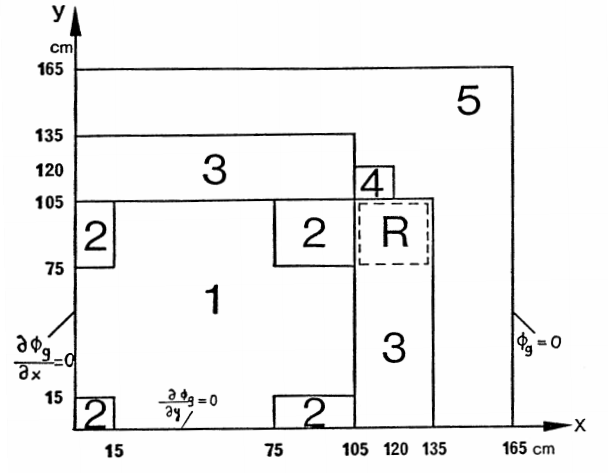
\includegraphics[width=0.8\linewidth]{\FiguresDir/lra.png}
\caption{LRA benchmark geometry with region assignment.}
\label{fig:lra-geometry}
\end{figure}

Initial two-group constants are presented in~\tbl{tab:lra-xs}.
$\nu$ is equal to 2.43.
Axial bulking $B^2 = 10^{-4}$ is applied for both energy groups.
Delayed neutron data are presented in~\tbl{tab:lra-dnp}.
All fuel materials have the same delayed neutron data.
Some scalar data are listed in~\tbl{tab:lra-scalar}.\\
\begin{table}[!htbp]
    \centering
    \caption{LRA benchmark initial two-group constants.\label{tab:lra-xs}}
    \resizebox{\textwidth}{!}{
      \begin{tabular}{|c|c|c|c|l|l|l|l|l|}
      \hline
             &                 & Group   & $D_g$      & $\Sigma_{a,g}$ & $\nu\Sigma_{f,g}$ & $\Sigma_{s,1\rightarrow 2}$ & $\chi_g$ & $v_g$              \\
      Region & Material        &       g & (cm)       &  ($cm^{-1}$)   &  ($cm^{-1}$)      &  ($cm^{-1}$)                &          & ($cm\cdot s^{-1}$) \\
      \hline
      1      & Fuel 1 with rod & 1       & 1.255      & 0.008252       & 0.004602          &                             & 1        & $3.0\times10^7$    \\
             &                 & 2       & 0.211      & 0.1003         & 0.1091            & 0.02533                     & 0        & $3.0\times10^5$    \\
      \hline
      2      & Fuel 1 without rod & 1    & 1.268      & 0.007181       & 0.004609          &                             & 1        & $3.0\times10^7$    \\
             &                    & 2    & 0.1902     & 0.07047        & 0.08675           & 0.02767                     & 0        & $3.0\times10^5$    \\
      \hline
      3      & Fuel 2 with rod & 1       & 1.259      & 0.008002       & 0.004663          &                             & 1        & $3.0\times10^7$    \\
             &                 & 2       & 0.2091     & 0.08344        & 0.1021            & 0.02617                     & 0        & $3.0\times10^5$    \\
      \hline
      4      & Fuel 2 without rod & 1    & 1.259      & 0.008002       & 0.004663          &                             & 1        & $3.0\times10^7$    \\
             &                    & 2    & 0.2091     & 0.073324       & 0.1021            & 0.02617                     & 0        & $3.0\times10^5$    \\
      \hline
      5      & Reflector        & 1      & 1.257      & 0.0006034      & -                 &                             & -        & $3.0\times10^7$    \\
             &                  & 2      & 0.1592     & 0.01911        & -                 & 0.04754                     & -        & $3.0\times10^5$    \\
      \hline
      \end{tabular}}
\end{table}

\begin{table}[!htbp]
    \centering
    \caption{LRA benchmark delayed neutron data.\label{tab:lra-dnp}}
      \begin{tabular}{|c|l|l|l|l|}
      \hline
      Group i & $\beta_i$ & $\lambda_i$ ($s^{-1}$) & $\chi_{d,i,1}$ & $\chi_{d,i,2}$ \\
      \hline
      1       & 0.0054    & 0.0654  & 1 & 0 \\
      2       & 0.001087  & 1.35    & 1 & 0 \\
      \hline
      \end{tabular}
\end{table}

\begin{table}[!htbp]
    \centering
    \caption{LRA benchmark scalar values.\label{tab:lra-scalar}}
      \begin{tabular}{|l|c|l|}
      \hline
      Meaning & Notation & value \\
      \hline
      Axial buckling for both energy groups & $B_g^2$  & $10^{-4}$ ($cm^{-2}$)\\
      Mean number of neutrons per fission   & $\nu$    & 2.43 \\
      Conversion factor                     & $\alpha$ & $3.83\times 10^{-11}$ ($K\cdot cm^{3}$) \\
      Feedback constant                     & $\gamma$ & $3.034\times 10^{-3}$ ($K^{1/2}$) \\
      Energy released per fission           & $\kappa$ & $3.204\times 10^{-11} $ ($J/fission$) \\
      Initial and reference temperature     & $T_0$    & 300 (K) \\
      Active core volume                    & $V_{core}$ & 17550 ($cm^2$)\\
      \hline
      \end{tabular}
\end{table}
The transient is initiated by changing the thermal absorption cross section as the following:
\begin{align}
\Sigma_{a,2}(t) = \Sigma_{a,2}(t=0) \left\{\begin{array}{lr} 1-0.0606184t, & t\leq 2 \\
                                                             0.8787631, & t>2
                                           \end{array}\right.
\end{align}
where $t$ is time in seconds.

\section{TREAT Transient-15 Problem}

\section{TREAT M8-CAL Problem}